% homework/hw12x/hw12x.tex
% Year 7 - Extra Homework 12: What's Left of 180?
%
% Goes out with Homework 12 (homework/hw12, None of the Seven), due the same
% day. The teacher asked (11 Nov 2026) for "an easier 8 page packet that is
% more focused on adding and subtracting (some decimals) and some simpler
% angle problems with straight lines and whatnot". So:
%   Part 1  X1-X13. Add and take away: number bonds, in your head, column
%           grids for whole numbers and decimals (Unit 4), bar models, number
%           walls, the words that choose add or take away, a walk, a shop,
%           Mr Bowen's wrong answers, and one calculation -> English.
%   Part 2  X14-X22. Angles that are a take-away: 180 on a straight line
%           (one angle, then two), straight or not, angles in words, crossing
%           lines, 360 round a point, two of Mr Bowen's things, his wrong
%           angle homework, and one calculation -> English.
% The title is the whole sheet: an angle on a straight line is what is left
% of 180. X7(d) (a bar model of 180 degrees) is the bridge between the parts.
%
% As with EX 3-11, nothing on the sheet says easy, basic, extra help or
% catch-up. The scaffold fades in each question: the first is done, the next
% is printed, the last is an empty frame. Orange box = write a 0 here.
% Question numbers are X1-X22, because Homework 12 uses A-D.
%
% Nothing untaught: column addition and subtraction; Unit 4 decimals (line
% up the points, fill with 0, 8 = 8.00); 5.1's 180 on a line and 360 round a
% point and the two steps; 5.2's vertically opposite angles; a square mark =
% 90. No negative numbers, no protractor, no calculator, no science (the one
% gecko in X9(c) is HW 12's, as a length).
% HW 12's numbers (B1: 100, 145, 33, 57, 124; A5: 250) are not reused.
%
% House style is shared: see homework/hw-style.tex. Method: the new-homework
% skill. Source is pure ASCII on purpose.
%
% Build:  pwsh .claude/skills/new-homework/scripts/build-hw.ps1 hw12x

\documentclass[12pt,a4paper]{article}

% -- Answer key switch -------------------------------------------------------
\newif\ifkey
\ifdefined\TEACHER\keytrue\else
  \keyfalse        % \keyfalse = student copy   |   \keytrue = teacher copy
\fi

% -- House style -------------------------------------------------------------
% homework/hw-style.tex
% Shared house style for every Year 7 homework packet. \input this from the
% packet file, right after \documentclass and the answer-key switch.
%
% Do not fork this file per packet. If a packet needs a different look, the
% question is whether every packet should have it.
%
% The choices here are deliberate and were arrived at by printing and looking:
%   * No solid dark banners. Every header is a light tint with a coloured spine
%     on the left, so colour reads clearly without flooding a school printer.
%   * No marks and no mark totals. These are practice, not exam papers.
%   * Lato at 12pt with open leading, plus mathastext so inline maths is Lato
%     too. Without mathastext every "-6 + 4" is Computer Modern serif and the
%     sheet looks half-typeset.
%   * Writing lines are spaced for Year 7 handwriting, not adult margin notes.
%   * Pages fill. \needspace is redefined below so a heading no longer drags
%     the page break up to itself, and every heading is glued to the box under
%     it. Packets built before 2026-09-30 were laid out under the old rules and
%     will reflow if rebuilt -- re-read every page if you rebuild one.
%
% Provides: \wlines \blank \tickbox \sep \qmk-free marks (none) \hwsection
% \qhead \expr, the workspace box, and the remember / wordhelp / activity /
% yourturn coloured boxes. Palette matches the lesson decks exactly.

% -- Packages ----------------------------------------------------------------
\usepackage[T1]{fontenc}
\usepackage[utf8]{inputenc}
\usepackage[default]{lato}
\usepackage[a4paper,top=1.7cm,bottom=1.7cm,left=2.0cm,right=2.0cm,headheight=15pt]{geometry}
\usepackage{amsmath,amssymb}
\usepackage{xcolor}
\usepackage[most]{tcolorbox}
\usepackage{enumitem}
\usepackage{tikz}
\usetikzlibrary{arrows.meta}
\usepackage{array}
\usepackage{tabularx}
\usepackage{fancyhdr}
\usepackage{multicol}
\usepackage{needspace}
\usepackage{graphicx}

% Make maths use Lato too. Without this, every "-6 + 4" on the page is set in
% Computer Modern serif and the sheet looks half-typeset. Must come last.
\usepackage[italic]{mathastext}

% -- \needspace, without the hole it used to leave ----------------------------
% needspace.sty writes "\vskip 0pt plus X \penalty-100" in front of every
% heading. A page that ends anywhere else is underfull with no stretch, so TeX
% scores it b=10000; a page that ends AT a heading gets that X of stretch and a
% finite badness, and wins. So any heading in roughly the bottom half of a page
% claimed the break, and the question under it moved over whole, leaving a hole
% the size of the question. \tracingpages showed it exactly (b=4531 at the
% heading, b=10000 at every later break) while building homework/q1rev, and it
% is where the half-empty pages in HW 1-8 came from.
% This keeps only the \penalty9999, which still refuses to put a heading in the
% last X of a page. Keeping a heading WITH the box under it is \nobreak's job
% now -- see \hwsection and \qhead below.
\makeatletter
\renewcommand{\needspace}[1]{\begingroup\setlength{\dimen@}{#1}%
  \vskip\dimen@\penalty9999\vskip-\dimen@\endgroup}
\makeatother

\linespread{1.06}\selectfont

% -- The Learner's Book palette (same hex values as the lesson decks) ---------
\definecolor{cbteal}{HTML}{0087A8}
\definecolor{cbpurple}{HTML}{5C2483}
\definecolor{cborange}{HTML}{C25E12}
\definecolor{cbgreen}{HTML}{4A8B23}
\definecolor{cbred}{HTML}{C8102E}
\definecolor{cbblue}{HTML}{1A5FA8}
\definecolor{rulegray}{HTML}{9AA5AD}

% -- Answer lines and blanks -------------------------------------------------
% \wlines{n} draws n ruled writing lines, spaced wide enough for Year 7
% handwriting rather than for an adult with a fine pen.
\makeatletter
\newcommand{\wlines}[1]{%
  \par\vspace{0.75em}%
  \@tempcnta=0\relax
  \@whilenum\@tempcnta<#1\do{%
    \hbox to \linewidth{\color{rulegray}\leaders\hrule height 0.5pt\hfill}%
    \vspace{1.5em}%
    \advance\@tempcnta by 1\relax}%
  \par\vspace{-0.8em}%
}
\makeatother

% \blank[width] is an inline gap to write a short answer in.
\newcommand{\blank}[1][2.6cm]{\underline{\hspace{#1}}}

% A boxed space for showing working.
\newtcolorbox{workspace}[1][3.4cm]{%
  colback=white, colframe=rulegray, boxrule=0.5pt, arc=5pt,
  height=#1, left=6pt, right=6pt, top=4pt, bottom=4pt,
  before skip=9pt, after skip=11pt}

% An empty tick box.
\newcommand{\tickbox}{\fbox{\rule{0pt}{1.15em}\rule{1.15em}{0pt}}}

% A middot separator.
\newcommand{\sep}{\,\textperiodcentered\,}

% -- Section and question headings -------------------------------------------
% Light tint plus a fat coloured spine on the left. No solid dark banner: the
% colour reads clearly but barely costs the printer anything.
% needspace keeps a heading out of the last few lines of a page. The \nobreak
% after it keeps it with whatever comes next: a remember or word-help box that
% does not fit takes its heading over with it, instead of leaving the heading
% alone at the foot of the page. (The old needspace did that by accident, and
% left a hole every time; see above.)
\newcommand{\hwsection}[2][cbteal]{%
  \needspace{8\baselineskip}%
  \par\vspace{13pt}%
  \noindent
  \begin{tcolorbox}[enhanced, nobeforeafter, width=\textwidth,
      colback=#1!7, colframe=#1!7, arc=5pt,
      borderline west={5pt}{0pt}{#1},
      left=14pt, right=10pt, top=7pt, bottom=7pt]
    {\large\bfseries\color{#1}#2}
  \end{tcolorbox}%
  \par\nobreak\vspace{9pt}}

% \qhead[colour]{A2}{Moving along the line} -- a question heading.
\newcommand{\qhead}[3][cbteal]{%
  \needspace{6\baselineskip}%
  \par\vspace{11pt}%
  \noindent{\large\bfseries\color{#1}#2}\quad{\large\bfseries #3}\par\nobreak\vspace{4pt}}

% -- Coloured boxes ----------------------------------------------------------
% Shared look: rounded, light fill, coloured rule, coloured title text on a
% pale title strip rather than a dark one.
% NOT breakable. A breakable box that cannot fit its first lines forces its own
% page break, and \nobreak cannot stop a forced break -- so the heading above
% it was left alone at the foot of the page (tested: it happens with \nobreak
% in place). Unbreakable, the page builder moves heading and box together.
% These boxes are a few lines each; none needs to split.
\tcbset{hwbox/.style={
  enhanced, arc=6pt, boxrule=1pt,
  left=11pt, right=11pt, top=8pt, bottom=8pt,
  fonttitle=\bfseries, attach boxed title to top left={xshift=12pt, yshift=-8pt},
  boxed title style={arc=4pt, boxrule=1pt, left=7pt, right=7pt, top=2pt, bottom=2pt},
  top=13pt}}

% Orange: things to remember. Matches the deck's "Write This Down".
\newtcolorbox{remember}[1][Remember from the lesson]{hwbox,
  colback=cborange!6, colframe=cborange, coltitle=cborange,
  colbacktitle=white, title={#1}}

% Blue: English help. The barrier in this class is the wording, not the maths.
\newtcolorbox{wordhelp}[1][Word help]{hwbox,
  colback=cbblue!6, colframe=cbblue, coltitle=cbblue,
  colbacktitle=white, title={#1}}

% Purple: an activity or instruction.
\newtcolorbox{activity}[1][How to do this homework]{hwbox,
  colback=cbpurple!6, colframe=cbpurple, coltitle=cbpurple,
  colbacktitle=white, title={#1}}

% Green: your turn / a friendly nudge.
\newtcolorbox{yourturn}[1][Your turn]{hwbox,
  colback=cbgreen!7, colframe=cbgreen, coltitle=cbgreen!75!black,
  colbacktitle=white, title={#1}}

% -- Shorthands --------------------------------------------------------------
\newcommand{\dC}{\,^{\circ}\mathrm{C}}          % use inside maths: $-8\dC$
\newcommand{\key}[1]{{\color{cborange}\textbf{#1}}}
\newcommand{\eng}[1]{{\color{cbblue}\textbf{#1}}}

\setlist[enumerate]{itemsep=8pt, topsep=5pt, leftmargin=*}
\setlist[itemize]{itemsep=4pt, topsep=4pt, leftmargin=*}
\renewcommand{\arraystretch}{1.45}

% -- An expression the student is asked to work from -------------------------
\newcommand{\expr}[1]{%
  \tcbox[on line, colback=cbgreen!10, colframe=cbgreen!55, boxrule=1pt, arc=4pt,
         left=9pt, right=9pt, top=4pt, bottom=4pt]{\large\bfseries $#1$}}

% -- Running head and foot ---------------------------------------------------
% The packet overrides \fancyhead[L] with its own title.
\pagestyle{fancy}
\fancyhf{}
\fancyhead[L]{\small\color{black!55}Year 7\sep Homework}
\fancyhead[R]{\small\color{black!55}Name: \blank[3.4cm]}
\fancyfoot[C]{\small\color{black!55}Page \thepage}
\renewcommand{\headrulewidth}{0pt}
\renewcommand{\headrule}{\vspace{2pt}\hbox to\headwidth{\color{cbteal!45}\leaders\hrule height 1.2pt\hfill}}


\usetikzlibrary{angles,quotes,calc}

% -- Per-packet running head -------------------------------------------------
\fancyhead[L]{\small\color{black!55}Year 7\sep Extra Homework 12}

% -- Degrees, inside maths: $72\dg$ ------------------------------------------
\newcommand{\dg}{^{\circ}}

% -- Small things to write in ------------------------------------------------
\newcommand{\nbox}{\ \fbox{\rule{0pt}{1.05em}\rule{1.0em}{0pt}}\ }
% teal, for the worked example
\newcommand{\tl}[1]{{\color{cbteal}\bfseries #1}}
% a blank with the worked answer in it
\newcommand{\done}[2][1.6cm]{\underline{\makebox[#1]{\color{cbteal}\bfseries #2}}}

% -- "Calculation: ____  Answer: ____" on a line of its own -------------------
\newcommand{\calcans}[1][6.6cm]{\par\nobreak\vspace{4pt}\noindent\hspace*{1.6em}%
  \textbf{Calculation:} \blank[#1] \hfill \textbf{Answer:} \blank[3.0cm]\par}

% -- A group of writing lines that will not be split -------------------------
\newcommand{\qlines}[1]{\par\nobreak
  \noindent\begin{minipage}{\linewidth}\wlines{#1}\end{minipage}\par}

% -- Columns -----------------------------------------------------------------
\newcolumntype{L}{>{\raggedright\arraybackslash}X}
\newcolumntype{C}[1]{>{\centering\arraybackslash\leavevmode}p{#1}}
\newcolumntype{P}[1]{>{\leavevmode\raggedright\arraybackslash}p{#1}}
\newcolumntype{W}[1]{>{\leavevmode\raggedright\bfseries\color{cbblue}}p{#1}}
\newcommand{\tall}{\rule[-0.6em]{0pt}{1.9em}}

% -- Angle drawing styles (as HW 11 and HW 12) --------------------------------
\tikzset{
  ang/.style={draw=cborange, line width=0.8pt, angle radius=0.5cm,
    angle eccentricity=1.75, pic text options={font=\small}},
  let/.style={draw=cbteal, line width=0.8pt, angle radius=0.42cm,
    angle eccentricity=2.2, pic text options={font=\small\bfseries\itshape, text=cbteal}},
  rt/.style={draw=black!70, line width=0.7pt, angle radius=0.25cm},
}

% ---------------------------------------------------------------------------
% COLUMN GRIDS (from EX 11). An entry is a digit, nothing, z (an orange box:
% write a 0 here) or Z (an orange box with the 0 already written).
% \colgrid{op}{row 1}{row 2}{answer}: tens, ones, POINT, tenths, hundredths.
% \wgrid{op}{carries}{row 1}{row 2}{answer}: hundreds, tens, ones, no point.
%   A carry entry is nothing, e (a small empty box) or a digit (a small box
%   with the digit in it, for the worked example).
% ---------------------------------------------------------------------------
\def\zz{z}
\def\ZZ{Z}
\def\ee{e}
\newcommand{\gcell}[4][black]{%
  \edef\gcE{#4}%
  \ifx\gcE\zz
    \filldraw[fill=cborange!14, draw=cborange!80, line width=0.8pt]
      (#2,#3) rectangle ++(0.72,0.78);
  \else\ifx\gcE\ZZ
    \filldraw[fill=cborange!14, draw=cborange!80, line width=0.8pt]
      (#2,#3) rectangle ++(0.72,0.78);
    \node[font=\large\bfseries, text=cborange] at (#2+0.36,#3+0.39) {0};
  \else
    \draw[rulegray, line width=0.6pt] (#2,#3) rectangle ++(0.72,0.78);
    \node[font=\large, text=#1] at (#2+0.36,#3+0.39) {\gcE};
  \fi\fi}
\newcommand{\ccell}[3]{%
  \edef\gcE{#3}%
  \ifx\gcE\empty\else
    \draw[rulegray, line width=0.5pt, densely dashed] (#1+0.18,#2) rectangle ++(0.36,0.36);
    \ifx\gcE\ee\else
      \node[font=\footnotesize\bfseries, text=cbteal] at (#1+0.36,#2+0.18) {\gcE};
    \fi
  \fi}
\newcommand{\colgrid}[4]{%
  \begin{tikzpicture}[x=1cm, y=1cm, baseline=(current bounding box.north)]
    \foreach \d [count=\i] in {#2}{%
      \pgfmathsetmacro\xx{(\i-1)*0.72+(\i>2)*0.30}\gcell{\xx}{1.75}{\d}}
    \foreach \d [count=\i] in {#3}{%
      \pgfmathsetmacro\xx{(\i-1)*0.72+(\i>2)*0.30}\gcell{\xx}{0.85}{\d}}
    \foreach \d [count=\i] in {#4}{%
      \pgfmathsetmacro\xx{(\i-1)*0.72+(\i>2)*0.30}\gcell[cbteal]{\xx}{-0.25}{\d}}
    \foreach \y in {1.75,0.85,-0.25}{\fill (1.59,\y+0.13) circle (0.06);}
    \node[font=\Large] at (-0.42,1.24) {$#1$};
    \draw[line width=1.2pt] (-0.75,0.72) -- (3.18,0.72);
  \end{tikzpicture}}
\newcommand{\wgrid}[5]{%
  \begin{tikzpicture}[x=1cm, y=1cm, baseline=(current bounding box.north)]
    \foreach \d [count=\i] in {#2}{%
      \pgfmathsetmacro\xx{(\i-1)*0.72}\ccell{\xx}{2.62}{\d}}
    \foreach \d [count=\i] in {#3}{%
      \pgfmathsetmacro\xx{(\i-1)*0.72}\gcell{\xx}{1.75}{\d}}
    \foreach \d [count=\i] in {#4}{%
      \pgfmathsetmacro\xx{(\i-1)*0.72}\gcell{\xx}{0.85}{\d}}
    \foreach \d [count=\i] in {#5}{%
      \pgfmathsetmacro\xx{(\i-1)*0.72}\gcell[cbteal]{\xx}{-0.25}{\d}}
    \node[font=\Large] at (-0.42,1.24) {$#1$};
    \draw[line width=1.2pt] (-0.75,0.72) -- (2.16,0.72);
  \end{tikzpicture}}

% -- Angle pictures ------------------------------------------------------------
% \lineone[side]{angle}{its label}{letter}: a straight line, one ray. The
% known angle is measured from the right and the letter is the rest, on the
% left; [L] swaps them. (Not xscale=-1: the angle pics always run
% anticlockwise, so a mirrored picture draws the reflex angle.)
\def\LL{L}
\newcommand{\lineone}[4][R]{%
  \begin{tikzpicture}[line width=1pt, baseline=(current bounding box.south)]
    \coordinate (O) at (0,0); \coordinate (L) at (-1.75,0); \coordinate (R) at (1.75,0);
    \def\gcE{#1}%
    \ifx\gcE\LL
      \coordinate (P) at ({180-#2}:1.55);
      \draw (L) -- (R); \draw (O) -- (P);
      \pic[ang, "#3"] {angle = P--O--L};
      \pic[let, "$#4$"] {angle = R--O--P};
    \else
      \coordinate (P) at (#2:1.55);
      \draw (L) -- (R); \draw (O) -- (P);
      \pic[ang, "#3"] {angle = R--O--P};
      \pic[let, "$#4$"] {angle = P--O--L};
    \fi
  \end{tikzpicture}}
% \linetwo{first ray}{first label}{second ray}{second label or RT}{letter}:
% two rays; the letter is what is left on the left. RT draws a right-angle
% square instead of a number.
\def\RT{RT}
\newcommand{\linetwo}[5]{%
  \begin{tikzpicture}[line width=1pt, baseline=(current bounding box.south)]
    \coordinate (O) at (0,0); \coordinate (L) at (-1.75,0); \coordinate (R) at (1.75,0);
    \coordinate (P) at (#1:1.55); \coordinate (Q) at (#3:1.55);
    \draw (L) -- (R); \draw (O) -- (P); \draw (O) -- (Q);
    \pic[ang, "#2", angle radius=0.62cm, angle eccentricity=1.6] {angle = R--O--P};
    \def\gcE{#4}%
    \ifx\gcE\RT \pic[rt] {right angle = P--O--Q};
    \else \pic[ang, "#4"] {angle = P--O--Q}; \fi
    \pic[let, "$#5$"] {angle = Q--O--L};
  \end{tikzpicture}}

% -- A bar model: \barm{whole}{part 1}{part 2}{width of part 1, cm} ----------
% The whole is 5.6 cm wide; part 1 is drawn to scale.
\newcommand{\barm}[4]{%
  \begin{tikzpicture}[font=\large]
    \draw[fill=cbgreen!12, draw=cbgreen!60!black, line width=0.8pt] (0,0.8) rectangle (5.6,1.5);
    \node at (2.8,1.15) {#1};
    \draw[fill=white, draw=cborange!75!black, line width=0.8pt] (0,0) rectangle (#4,0.7);
    \node at ({#4/2},0.35) {#2};
    \draw[fill=white, draw=cborange!75!black, line width=0.8pt] (#4,0) rectangle (5.6,0.7);
    \node at ({(#4+5.6)/2},0.35) {#3};
  \end{tikzpicture}}
\newcommand{\q}{{\color{cborange}\bfseries ?}}

\begin{document}

% ===========================================================================
% COVER BLOCK
% ===========================================================================
\thispagestyle{fancy}

\begin{tcolorbox}[enhanced, colback=cbgreen!8, colframe=cbgreen!8, arc=7pt,
                  borderline west={6pt}{0pt}{cbgreen},
                  left=18pt, right=14pt, top=11pt, bottom=11pt]
  {\color{cbgreen!75!black}\bfseries YEAR 7\sep MATHS UNITS 4 AND 5\sep
  EXTRA HOMEWORK 12}\\[6pt]
  {\color{cbgreen!70!black}\Huge\bfseries What's Left of 180\textdegree?}\\[10pt]
  {\color{black!70}Add and take away\sep decimals\sep a walk and a shop\sep angles on
  a straight line}
\end{tcolorbox}

\vspace{6pt}
\noindent
\begin{tabularx}{\textwidth}{@{}X X@{}}
  \textbf{Name:} \blank[5.6cm] & \textbf{Class:} \blank[5.6cm] \\
  \textbf{Date given:} \blank[4.6cm] &
  \textbf{Date due:} {\color{cbred}\bfseries Monday 16 November 2026} \\
\end{tabularx}

\vspace{4pt}
\begin{activity}[Why this sheet exists]
  Every question here is an \key{add} or a \key{take away} --- the angles too. An
  angle on a straight line is what is left of \key{180\textdegree}.

  \medskip
  The steps are printed as \key{boxes}. Fill the boxes --- that \emph{is} the method.
  An \key{orange box} means: write a \key{0} here.

  \medskip
  \eng{No calculator. No protractor.} \; Write the \key{calculation} first, then the
  answer.
\end{activity}

% ===========================================================================
% PART 1 -- ADD AND TAKE AWAY
% ===========================================================================
\hwsection[cbgreen]{Part 1 \textperiodcentered\ Add and take away}

% -- X1 ---------------------------------------------------------------------
% The way in: number bonds, and the two that the angles need (180 and 360).
\qhead[cbgreen]{X1}{Make the total}

\noindent\begin{minipage}{\textwidth}
\noindent Write the missing number. (a) is done for you.

\vspace{4pt}
{\renewcommand{\arraystretch}{2.0}%
\noindent\begin{tabularx}{\textwidth}{@{}L L L@{}}
  \textbf{(a)} \ $7 + {}$\done[1.3cm]{3}${} = 10$ &
  \textbf{(b)} \ $60 + {}$\blank[1.3cm]${} = 100$ &
  \textbf{(c)} \ $35 + {}$\blank[1.3cm]${} = 100$ \\
  \textbf{(d)} \ $0.4 + {}$\blank[1.3cm]${} = 1$ &
  \textbf{(e)} \ $0.75 + {}$\blank[1.3cm]${} = 1$ &
  \textbf{(f)} \ $100 + {}$\blank[1.3cm]${} = 180$ \\
  \textbf{(g)} \ $130 + {}$\blank[1.3cm]${} = 180$ &
  \textbf{(h)} \ $95 + {}$\blank[1.3cm]${} = 180$ &
  \textbf{(i)} \ $270 + {}$\blank[1.3cm]${} = 360$ \\
\end{tabularx}}
\end{minipage}

% -- X2 ---------------------------------------------------------------------
% In your head: tenths that make a whole, and take-aways from whole numbers
% that leave a decimal. (k) and (l) are the angle facts again.
\qhead[cbgreen]{X2}{In your head}

\noindent\begin{minipage}{\textwidth}
\noindent No column grid this time. (a) is done for you.

\vspace{4pt}
{\renewcommand{\arraystretch}{2.0}%
\noindent\begin{tabularx}{\textwidth}{@{}L L L@{}}
  \textbf{(a)} \ $0.5 + 0.5 = {}$\done[1.4cm]{1} &
  \textbf{(b)} \ $1.2 + 0.8 = {}$\blank[1.4cm] &
  \textbf{(c)} \ $2.5 + 2.5 = {}$\blank[1.4cm] \\
  \textbf{(d)} \ $4.6 + 0.4 = {}$\blank[1.4cm] &
  \textbf{(e)} \ $0.9 + 0.2 = {}$\blank[1.4cm] &
  \textbf{(f)} \ $3 - 0.5 = {}$\blank[1.4cm] \\
  \textbf{(g)} \ $10 - 0.1 = {}$\blank[1.4cm] &
  \textbf{(h)} \ $1 - 0.25 = {}$\blank[1.4cm] &
  \textbf{(i)} \ $7.5 - 2.5 = {}$\blank[1.4cm] \\
  \textbf{(j)} \ $6 - 1.5 = {}$\blank[1.4cm] &
  \textbf{(k)} \ $180 - 90 = {}$\blank[1.4cm] &
  \textbf{(l)} \ $360 - 180 = {}$\blank[1.4cm] \\
\end{tabularx}}
\end{minipage}

% -- X3 ---------------------------------------------------------------------
% Column addition, whole numbers. (a) done with its carry; (b) printed;
% (c) empty: the student places 96 under 409 (ones under ones).
\qhead[cbgreen]{X3}{Add in columns}

\noindent\begin{minipage}{\textwidth}
\noindent A carried 1 goes in the small dashed box. In (c), write the numbers in the
grid yourself.

\vspace{6pt}
\noindent
\begin{minipage}[t]{0.32\textwidth}\centering
  \textbf{(a)} \ $246 + 137$ \ done\par\vspace{4pt}
  \wgrid{+}{,1,}{2,4,6}{1,3,7}{3,8,3}
\end{minipage}\hfill
\begin{minipage}[t]{0.32\textwidth}\centering
  \textbf{(b)} \ $358 + 275$\par\vspace{4pt}
  \wgrid{+}{e,e,e}{3,5,8}{2,7,5}{,,}
\end{minipage}\hfill
\begin{minipage}[t]{0.32\textwidth}\centering
  \textbf{(c)} \ $409 + 96$\par\vspace{4pt}
  \wgrid{+}{e,e,e}{,,}{,,}{,,}
\end{minipage}
\end{minipage}

% -- X4 ---------------------------------------------------------------------
% Column subtraction, whole numbers. (b) and (c) are the take-aways the angles
% need: 180 and 360.
\qhead[cbgreen]{X4}{Take away in columns}

\noindent\begin{minipage}{\textwidth}
\noindent The first number goes on top. In (c), write the numbers in the grid yourself.

\vspace{6pt}
\noindent
\begin{minipage}[t]{0.32\textwidth}\centering
  \textbf{(a)} \ $452 - 128$ \ done\par\vspace{4pt}
  \wgrid{-}{,,}{4,5,2}{1,2,8}{3,2,4}
\end{minipage}\hfill
\begin{minipage}[t]{0.32\textwidth}\centering
  \textbf{(b)} \ $180 - 74$\par\vspace{4pt}
  \wgrid{-}{,,}{1,8,0}{,7,4}{,,}
\end{minipage}\hfill
\begin{minipage}[t]{0.32\textwidth}\centering
  \textbf{(c)} \ $360 - 145$\par\vspace{4pt}
  \wgrid{-}{,,}{,,}{,,}{,,}
\end{minipage}
\end{minipage}

% -- X5 ---------------------------------------------------------------------
% Decimals: line up the points, fill with 0. (a) done; (b) printed with its
% orange box; (c) empty, and it needs the tens column.
\qhead[cbgreen]{X5}{Add decimals}

\begin{remember}[Remember from Unit 4]
  \key{Line up the points.} The point is printed in every row --- it cannot move. \\
  An empty place gets a \key{0}: \ $2.3 = 2.30$ \quad and \quad $8 = 8.00$.
\end{remember}

\noindent\begin{minipage}{\textwidth}
\noindent
\begin{minipage}[t]{0.32\textwidth}\centering
  \textbf{(a)} \ $3.45 + 2.3$ \ done\par\vspace{4pt}
  \colgrid{+}{,3,4,5}{,2,3,Z}{,5,7,5}
\end{minipage}\hfill
\begin{minipage}[t]{0.32\textwidth}\centering
  \textbf{(b)} \ $4.7 + 1.85$\par\vspace{4pt}
  \colgrid{+}{,4,7,z}{,1,8,5}{,,,}
\end{minipage}\hfill
\begin{minipage}[t]{0.32\textwidth}\centering
  \textbf{(c)} \ $12.6 + 0.75$\par\vspace{4pt}
  \colgrid{+}{,,,}{,,,}{,,,}
\end{minipage}
\end{minipage}

% -- X6 ---------------------------------------------------------------------
% (c) is the one that matters: 8 - 3.25, where 8 = 8.00 and both orange boxes
% are needed. The usual wrong answer is 5.25 (8 - 3, keep the .25).
\qhead[cbgreen]{X6}{Take away decimals}

\noindent\begin{minipage}{\textwidth}
\noindent In (d), write the numbers in the grid yourself.

\vspace{6pt}
\noindent
\begin{minipage}[t]{0.24\textwidth}\centering
  \textbf{(a)} \ $5.6 - 2.35$ \ done\par\vspace{4pt}
  \colgrid{-}{,5,6,Z}{,2,3,5}{,3,2,5}
\end{minipage}\hfill
\begin{minipage}[t]{0.24\textwidth}\centering
  \textbf{(b)} \ $7.4 - 3.18$\par\vspace{4pt}
  \colgrid{-}{,7,4,z}{,3,1,8}{,,,}
\end{minipage}\hfill
\begin{minipage}[t]{0.24\textwidth}\centering
  \textbf{(c)} \ $8 - 3.25$\par\vspace{4pt}
  \colgrid{-}{,8,z,z}{,3,2,5}{,,,}
\end{minipage}\hfill
\begin{minipage}[t]{0.24\textwidth}\centering
  \textbf{(d)} \ $10 - 4.6$\par\vspace{4pt}
  \colgrid{-}{,,,}{,,,}{,,,}
\end{minipage}
\end{minipage}

% -- X7 ---------------------------------------------------------------------
% Bar models: the picture chooses the operation. A missing whole is an add; a
% missing part is a take-away. (d) is the bridge to Part 2: the whole is 180.
\qhead[cbgreen]{X7}{Bar models}

\begin{remember}[How a bar model works]
  The long bar on top is the \key{whole}. The two bars under it are the \key{parts}.
  \\ Whole missing? \ \key{Add} the parts. \qquad A part missing? \ \key{Take away}:
  whole $-$ part.
\end{remember}

\noindent\begin{minipage}{\textwidth}
\noindent Find each \q. (a) is done for you.

\vspace{6pt}
\noindent
\begin{minipage}[t]{0.48\textwidth}\centering
  \textbf{(a)}\par\vspace{2pt}\barm{\q}{2.4}{1.5}{3.45}
  \par\vspace{6pt}\raggedright\hspace*{0.6em}\textbf{Calculation:}
  \tl{$2.4 + 1.5 = 3.9$} \ \ \q\ $=$ \done[1.2cm]{3.9}
\end{minipage}\hfill
\begin{minipage}[t]{0.48\textwidth}\centering
  \textbf{(b)}\par\vspace{2pt}\barm{6.0}{3.8}{\q}{3.55}
  \par\vspace{6pt}\raggedright\hspace*{0.6em}\textbf{Calculation:} \blank[2.6cm] \ \
  \q\ $=$ \blank[1.2cm]
\end{minipage}

\vspace{12pt}
\noindent
\begin{minipage}[t]{0.48\textwidth}\centering
  \textbf{(c)}\par\vspace{2pt}\barm{\q}{0.75}{1.25}{2.1}
  \par\vspace{6pt}\raggedright\hspace*{0.6em}\textbf{Calculation:} \blank[2.6cm] \ \
  \q\ $=$ \blank[1.2cm]
\end{minipage}\hfill
\begin{minipage}[t]{0.48\textwidth}\centering
  \textbf{(d)}\par\vspace{2pt}\barm{180\textdegree}{65\textdegree}{\q}{2.0}
  \par\vspace{6pt}\raggedright\hspace*{0.6em}\textbf{Calculation:} \blank[2.6cm] \ \
  \q\ $=$ \blank[1.2cm]
\end{minipage}
\end{minipage}

% -- X8 ---------------------------------------------------------------------
% Number walls: each brick is the two under it added. Wall 1 is all adding.
% Wall 2 has a missing bottom brick, so it starts with a take-away:
% 4.25 - 1.5 = 2.75.
\qhead[cbgreen]{X8}{Number walls}

\newcommand{\brick}[3]{%
  \draw[cborange!70!black, line width=0.8pt, fill=white] (#1,#2) rectangle ++(1.5,0.8);
  \node[font=\large] at (#1+0.75,#2+0.4) {#3};}
\noindent\begin{minipage}{\textwidth}
\noindent Each brick is the \textbf{two bricks under it, added}. Fill every empty brick.

\vspace{6pt}
\noindent
\begin{minipage}[c]{0.52\textwidth}\centering
  
\begin{tikzpicture}
    \brick{0}{0}{12}\brick{1.5}{0}{25}\brick{3}{0}{8}\brick{4.5}{0}{30}
    \brick{0.75}{0.8}{\color{cbteal}\bfseries 37}\brick{2.25}{0.8}{}\brick{3.75}{0.8}{}
    \brick{1.5}{1.6}{}\brick{3}{1.6}{}
    \brick{2.25}{2.4}{}
    \node[font=\small\bfseries, anchor=east] at (-0.1,0.4) {(a)};
  \end{tikzpicture}
\end{minipage}\hfill
\begin{minipage}[c]{0.46\textwidth}\centering
  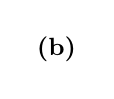
\begin{tikzpicture}
    \brick{0}{0}{1.5}\brick{1.5}{0}{}\brick{3}{0}{2.25}
    \brick{0.75}{0.8}{4.25}\brick{2.25}{0.8}{}
    \brick{1.5}{1.6}{}
    \node[font=\small\bfseries, anchor=east] at (-0.1,0.4) {(b)};
  \end{tikzpicture}
  \par\vspace{4pt}{\small A bottom brick is missing: \ $1.5 + {?} = 4.25$. \ Take
  away.}
\end{minipage}
\end{minipage}

% -- X9 ---------------------------------------------------------------------
% THE LANGUAGE QUESTION. Each English phrase chooses add or take away.
% (c) is the gecko from HW 12's C2, growing. (f) is "subtract X from Y".
\qhead[cbgreen]{X9}{Add or take away?}

\begin{wordhelp}[Word help --- which one?]
  \renewcommand{\arraystretch}{1.25}%
  \begin{tabularx}{\linewidth}{@{}W{2.4cm}L@{}}
    add & total \sep altogether \sep the sum of \sep more (it grows) \\
    take away & the difference between \sep how much more \sep change \sep left
      \sep subtract \\
  \end{tabularx}
  \par\vspace{3pt}\noindent \textbf{Careful:} \ \emph{subtract 2 from 9} \ means \
  $9 - 2$. \ The second number comes first.
\end{wordhelp}

\noindent Write the \textbf{calculation first}. Then write the answer.

\begin{enumerate}[label=(\alph*), itemsep=5pt]
  \item What is the total of 2.5 and 1.25?
        \calcans
  \item What is the difference between 9.6 and 4.2?
        \calcans
  \item A gecko is 4.5 cm long. It grows 1.8 cm. How long is it now?
        \calcans
  \item A bottle holds 1.5 litres of water. Mr Bowen drinks 0.35 litres. How much is
        left?
        \calcans
  \item Mr Bowen walks 2.4 km on Monday and 3.15 km on Tuesday. How far does he walk
        altogether?
        \calcans
  \item Subtract 2.7 from 6.
        \calcans
\end{enumerate}

% -- X10 --------------------------------------------------------------------
% A map, drawn to scale (1 km = 4 cm). (b) "how much longer" is a take-away;
% (d) is four adds and deadpan.
\qhead[cbgreen]{X10}{Mr Bowen's walk to school}

\noindent\begin{minipage}{\textwidth}
\noindent Mr Bowen walks to school. He can go past the shop, or along the river.

\vspace{6pt}
\begin{center}
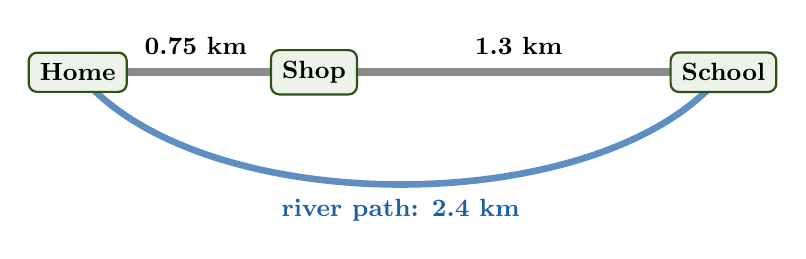
\begin{tikzpicture}[font=\small]
  \draw[cbblue!70, line width=2.4pt] (0,0) .. controls (1.5,-1.9) and (6.7,-1.9) .. (8.2,0);
  \node[text=cbblue, font=\small\bfseries] at (4.1,-1.75) {river path: 2.4 km};
  \draw[black!45, line width=3pt] (0,0) -- (8.2,0);
  \node[above=3pt, font=\small\bfseries] at (1.5,0) {0.75 km};
  \node[above=3pt, font=\small\bfseries] at (5.6,0) {1.3 km};
  \foreach \x/\n in {0/Home, 3/Shop, 8.2/School}
    \node[draw=cbgreen!60!black, fill=cbgreen!10, rounded corners=3pt, line width=0.8pt,
      font=\small\bfseries, inner sep=4pt] at (\x,0) {\n};
\end{tikzpicture}
\end{center}
\end{minipage}

\begin{enumerate}[label=(\alph*), itemsep=5pt]
  \item How far is it from home to school, past the shop?
        \calcans
  \item How much longer is the river path?
        \calcans
  \item He walks to school and home again, past the shop both times. How far does he
        walk altogether?
        \calcans
  \item One day he gets to the shop and remembers his laptop is at home. He walks home,
        back to the shop, and on to school. How far does he walk that morning?
        \calcans[8.4cm]
\end{enumerate}

% -- X11 --------------------------------------------------------------------
% Money, in dollars. (d) is two steps -- add, then take away -- the same two
% steps as the angles in Part 2.
\qhead[cbgreen]{X11}{Mr Bowen goes shopping}

% The price board sits beside (a)-(c), so the prices are never on one page
% and the questions on the next.
\newcommand{\shopq}[2]{%
  \textbf{#1} #2\par\nobreak\vspace{6pt}%
  \hspace*{1.2em}\textbf{Calculation:} \blank[3.4cm] \ \textbf{Answer:} \blank[1.7cm]\par
  \vspace{9pt}}
\noindent\begin{minipage}{\textwidth}
\noindent\begin{minipage}[t]{0.33\textwidth}\vspace{0pt}
  \begin{tcolorbox}[enhanced, colback=cbgreen!6, colframe=cbgreen!70!black,
                    boxrule=1pt, arc=6pt, left=8pt, right=8pt, top=4pt, bottom=4pt,
                    nobeforeafter, title={\bfseries School shop}, fonttitle=\small,
                    colbacktitle=cbgreen!70!black, coltitle=white]
    {\renewcommand{\arraystretch}{1.25}%
    \begin{tabular}{@{}l r@{}}
      notebook & 2.50 dollars \\
      pen & 1.25 dollars \\
      ruler & 0.80 dollars \\
      eraser & 0.45 dollars \\
      glue & 1.60 dollars \\
    \end{tabular}}
  \end{tcolorbox}
  \par\vspace{6pt}{\small\raggedright\eng{change}: the money you get back. You pay 5
  dollars, it costs 3 dollars: your change is $5 - 3 = 2$ dollars.\par}
\end{minipage}\hfill
\begin{minipage}[t]{0.63\textwidth}\vspace{0pt}\raggedright
  \shopq{(a)}{Mr Bowen buys a pen and a ruler. What is the total?}
  \shopq{(b)}{He buys a notebook. He pays with 5 dollars. What is his change?}
  \shopq{(c)}{How much more is the glue than the ruler?}
\end{minipage}
\end{minipage}

\vspace{8pt}
\noindent\begin{minipage}{\textwidth}
\noindent\textbf{(d)} He buys a notebook, a pen and an eraser. He pays with 5 dollars.
What is his change? \ Two steps:

\vspace{6pt}
{\renewcommand{\arraystretch}{1.9}%
\noindent\begin{tabular}{@{\hspace{1.6em}}l l@{}}
  \textbf{Step 1} \ add: & \blank[1.4cm] ${}+{}$ \blank[1.4cm] ${}+{}$ \blank[1.4cm]
    ${}={}$ \blank[1.8cm] \\
  \textbf{Step 2} \ take away: & $5.00 - {}$ \blank[1.8cm] ${}={}$ \blank[1.8cm]
    \ dollars \\
\end{tabular}}
\end{minipage}

% -- X12 --------------------------------------------------------------------
% The four errors a class makes with decimals. (c) is right, so a student
% cannot mark them all wrong.
\qhead[cbgreen]{X12}{Mr Bowen's homework}

\noindent\begin{minipage}{\textwidth}
\noindent Circle \textbf{right} or \textbf{wrong}. If it is wrong, write the correct
answer. Check with a column grid if you need to.

\vspace{6pt}
{\renewcommand{\arraystretch}{2.0}%
\noindent\begin{tabularx}{\textwidth}{@{}l L C{3.2cm} l@{}}
  \textbf{(a)} & $4.5 + 2.35 = 2.80$ & right \sep wrong & correct: \blank[2.4cm] \\
  \textbf{(b)} & $6 - 2.4 = 4.4$ & right \sep wrong & correct: \blank[2.4cm] \\
  \textbf{(c)} & $3.7 + 1.5 = 5.2$ & right \sep wrong & correct: \blank[2.4cm] \\
  \textbf{(d)} & $9 - 3.25 = 6.25$ & right \sep wrong & correct: \blank[2.4cm] \\
\end{tabularx}}

\vspace{6pt}
\noindent Choose \textbf{one} wrong answer. What did Mr Bowen do wrong? \\[3pt]
Start: \eng{``In (\ \ ), Mr Bowen \ldots''}
\qlines{2}
\end{minipage}

% -- X13 --------------------------------------------------------------------
% Calculation -> English: the best critical-thinking question in the format.
% Change from 5 dollars.
\qhead[cbgreen]{X13}{Now you write the question}

\noindent\begin{minipage}{\textwidth}
\noindent Write a word problem for \quad \expr{5.00 - 3.45 = 1.55}

\begin{yourturn}[Your word problem must have: tick each one]
  \renewcommand{\arraystretch}{1.35}%
  \begin{tabularx}{\linewidth}{@{}p{0.75cm}L p{0.75cm}L p{0.75cm}L@{}}
    \tickbox & Mr Bowen and a real thing to buy & \tickbox & the word
      \textbf{change} & \tickbox & dollars \\
    \tickbox & full sentences & \tickbox & a question at the end & \tickbox & the
      answer 1.55 dollars \\
  \end{tabularx}
\end{yourturn}
\wlines{4}
\end{minipage}

% ===========================================================================
% PART 2 -- ANGLES ON A STRAIGHT LINE
% ===========================================================================
\hwsection[cbgreen]{Part 2 \textperiodcentered\ Angles: what is left?}

% -- X14 --------------------------------------------------------------------
% One known angle on a straight line: 180 take away. (f) is a decimal, the
% same take-away as X6. The remember box, the instruction and the first row
% are one block, so the box never ends a page without its diagrams.
\qhead[cbgreen]{X14}{What is left of 180\textdegree?}

\newcommand{\xten}[2]{%
  \begin{minipage}[b]{0.315\textwidth}\centering
    #1\par\vspace{6pt}#2
  \end{minipage}}

\noindent\begin{minipage}{\textwidth}
\begin{remember}[Remember from 5.1]
  Angles on a \key{straight line} add up to \key{180\textdegree}. \quad
  A small square means a \key{right angle}: \key{90\textdegree}. \\
  Angles \key{around a point} add up to \key{360\textdegree}.
\end{remember}

\noindent Find each letter. Take the angle away from 180\textdegree. (a) is done for
you.

\vspace{6pt}
\noindent
\xten{\lineone{50}{$50\dg$}{a}}{\textbf{(a)} \ $180 - 50 = {}$\done[1.3cm]{130\textdegree}}\hfill
\xten{\lineone{110}{$110\dg$}{b}}{\textbf{(b)} \ $180 - {}$\blank[1.2cm]${} = {}$\blank[1.3cm]}\hfill
\xten{\lineone[L]{72}{$72\dg$}{c}}{\textbf{(c)} \ $180 - {}$\blank[1.2cm]${} = {}$\blank[1.3cm]}
\end{minipage}

\vspace{12pt}
\noindent\begin{minipage}{\textwidth}
\noindent
\xten{\lineone{145}{$145\dg$}{d}}{\textbf{(d)} \ $180 - {}$\blank[1.2cm]${} = {}$\blank[1.3cm]}\hfill
\xten{\lineone[L]{125}{$125\dg$}{e}}{\textbf{(e)} \ \blank[1.2cm]${} - {}$\blank[1.2cm]${} = {}$\blank[1.3cm]}\hfill
\xten{\lineone{147.5}{$147.5\dg$}{f}}{\textbf{(f)} \ \blank[3.4cm]}
\end{minipage}

% -- X15 --------------------------------------------------------------------
% Two angles on a line: add, then take away (the shopping's two steps).
% (b) has a right angle as a square, not a number.
\qhead[cbgreen]{X15}{Two angles, then what is left}

\newcommand{\xel}[2]{%
  \begin{minipage}[b]{0.315\textwidth}\centering
    #1\par\vspace{6pt}
    {\renewcommand{\arraystretch}{1.7}\begin{tabular}{@{}l@{\ }l@{}}#2\end{tabular}}
  \end{minipage}}

\noindent\begin{minipage}{\textwidth}
\noindent Step 1: \key{add} the two angles. \ Step 2: \key{take away} from
180\textdegree. (a) is done for you.

\vspace{6pt}
\noindent
\xel{\linetwo{40}{$40\dg$}{100}{$60\dg$}{p}}{%
  \textbf{1.} & \tl{$40 + 60 = 100$} \\
  \textbf{2.} & \tl{$180 - 100 = 80$} \\
  $p =$ & \tl{$80\dg$} \\}\hfill
\xel{\linetwo{35}{$35\dg$}{125}{RT}{q}}{%
  \textbf{1.} & \blank[3.0cm] \\
  \textbf{2.} & \blank[3.0cm] \\
  $q =$ & \blank[1.8cm] \\}\hfill
\xel{\linetwo{48}{$48\dg$}{123}{$75\dg$}{r}}{%
  \textbf{1.} & \blank[3.0cm] \\
  \textbf{2.} & \blank[3.0cm] \\
  $r =$ & \blank[1.8cm] \\}
\end{minipage}

% -- X16 --------------------------------------------------------------------
% Add, and look at the total: only exactly 180 is a straight line. 72 + 106
% looks straight and is not (the 5.1 vote again).
\qhead[cbgreen]{X16}{Straight line or not?}

\noindent\begin{minipage}{\textwidth}
\noindent Two angles sit side by side. Add them. Do they make a \textbf{straight
line}? Row 1 is done for you.

\vspace{4pt}
{\renewcommand{\arraystretch}{1.35}%
\noindent\begin{tabularx}{\textwidth}{|C{3.6cm}|L|C{3.0cm}|}
  \hline
  \textbf{The two angles} & \textbf{Add them} & \textbf{Straight line?} \\ \hline
  $95\dg$ and $85\dg$ \tall & \leavevmode{\color{cbteal}$95 + 85 = 180\dg$} &
    {\color{cbteal}yes} \\ \hline
  $72\dg$ and $106\dg$ \tall & & yes \sep no \\ \hline
  $129\dg$ and $51\dg$ \tall & & yes \sep no \\ \hline
  $88.5\dg$ and $91.5\dg$ \tall & & yes \sep no \\ \hline
  $64\dg$ and $117\dg$ \tall & & yes \sep no \\ \hline
\end{tabularx}}
\end{minipage}

% -- X17 --------------------------------------------------------------------
% Angles in words, no pictures: the English chooses 180, 90 or 360. (b) is
% "equal" (a divide by 2, the only one); (e) is a full turn.
\qhead[cbgreen]{X17}{Angles in words}

\begin{wordhelp}[Word help]
  \renewcommand{\arraystretch}{1.2}%
  \begin{tabularx}{\linewidth}{@{}W{2.7cm}L W{4.9cm}L@{}}
    straight line & 180\textdegree & full turn, around a point & 360\textdegree \\
    right angle & 90\textdegree & equal & the same size \\
  \end{tabularx}
\end{wordhelp}

\noindent You can draw a sketch. Write the \textbf{calculation first}.

\begin{enumerate}[label=(\alph*), itemsep=5pt]
  \item Two angles make a straight line. One of them is 70\textdegree. What is the
        other one?
        \calcans
  \item Two angles make a straight line. They are equal. How big is each one?
        \calcans
  \item Three angles make a straight line. Two of them are 50\textdegree\ and
        60\textdegree. What is the third?
        \calcans
  \item A right angle and one more angle make a straight line. How big is the other
        angle?
        \calcans
  \item Two angles make a full turn. One of them is 200\textdegree. What is the other?
        \calcans
\end{enumerate}

% -- X18 --------------------------------------------------------------------
% Two lines cross: opposite angles are equal, next-door angles make 180.
% (a) gives the opposite one; (b) gives nothing but the one angle.
\qhead[cbgreen]{X18}{Two lines cross}

\newcommand{\cross}[3]{% angle, its label, letters (three, comma-separated)
  \begin{tikzpicture}[line width=1pt]
    \coordinate (O) at (0,0);
    \coordinate (A1) at (0:1.7); \coordinate (A2) at (180:1.7);
    \coordinate (B1) at (#1:1.7); \coordinate (B2) at (#1+180:1.7);
    \draw (A2) -- (A1); \draw (B2) -- (B1);
    \pic[ang, "#2", angle radius=0.5cm, angle eccentricity=1.8] {angle = A1--O--B1};
    \foreach \l [count=\k] in {#3} {
      \ifnum\k=1 \pic[let, "$\l$", angle eccentricity=1.9] {angle = B1--O--A2};\fi
      \ifnum\k=2 \pic[let, "$\l$", angle eccentricity=1.9] {angle = A2--O--B2};\fi
      \ifnum\k=3 \pic[let, "$\l$", angle eccentricity=1.9] {angle = B2--O--A1};\fi}
  \end{tikzpicture}}

\noindent\begin{minipage}{\textwidth}
\begin{remember}[Remember from 5.2]
  When two lines cross, \key{opposite} angles are \key{equal}. \ Angles \key{next to}
  each other make a straight line: \key{180\textdegree}.
\end{remember}

\noindent
\begin{minipage}[c]{0.27\textwidth}\centering
  \cross{40}{$40\dg$}{s,t,u}\par\vspace{2pt}\textbf{(a)}
\end{minipage}\hfill
\begin{minipage}[c]{0.21\textwidth}
  {\renewcommand{\arraystretch}{1.7}%
  \begin{tabular}{@{}l@{\ }l@{}}
    $t =$ & \done[1.5cm]{40\textdegree} \\
    $s =$ & \blank[1.5cm] \\
    $u =$ & \blank[1.5cm] \\
  \end{tabular}}
\end{minipage}\hfill
\begin{minipage}[c]{0.27\textwidth}\centering
  \cross{115}{$115\dg$}{v,w,x}\par\vspace{2pt}\textbf{(b)}
\end{minipage}\hfill
\begin{minipage}[c]{0.21\textwidth}
  {\renewcommand{\arraystretch}{1.7}%
  \begin{tabular}{@{}l@{\ }l@{}}
    $v =$ & \blank[1.5cm] \\
    $w =$ & \blank[1.5cm] \\
    $x =$ & \blank[1.5cm] \\
  \end{tabular}}
\end{minipage}
\end{minipage}

% -- X19 --------------------------------------------------------------------
% Round a point: 360 take away. The same two steps.
\qhead[cbgreen]{X19}{Around a point}

\newcommand{\pointthree}[5]{% ray 2, label 1, ray 3, label 2, letter
  \begin{tikzpicture}[line width=1pt]
    \coordinate (O) at (0,0); \coordinate (R) at (0:1.6);
    \coordinate (P) at (#1:1.6); \coordinate (Q) at (#3:1.6);
    \draw (O) -- (R); \draw (O) -- (P); \draw (O) -- (Q);
    \def\gcE{#2}%
    \ifx\gcE\RT \pic[rt] {right angle = R--O--P};
    \else \pic[ang, "#2", angle eccentricity=1.9] {angle = R--O--P}; \fi
    \pic[ang, "#4", angle eccentricity=1.9] {angle = P--O--Q};
    \pic[let, "$#5$", angle eccentricity=1.9] {angle = Q--O--R};
    \fill (O) circle (1.6pt);
  \end{tikzpicture}}

\noindent\begin{minipage}{\textwidth}
\noindent Step 1: add the angles you know. \ Step 2: take away from \key{360\textdegree}.

\vspace{6pt}
\noindent
\begin{minipage}[c]{0.24\textwidth}\centering
  \pointthree{150}{$150\dg$}{275}{$125\dg$}{y}\par\textbf{(a)}
\end{minipage}\hfill
\begin{minipage}[c]{0.24\textwidth}
  {\renewcommand{\arraystretch}{1.7}%
  \begin{tabular}{@{}l@{\ }l@{}}
    \textbf{1.} & \blank[2.4cm] \\
    \textbf{2.} & \blank[2.4cm] \\
    $y =$ & \blank[1.5cm] \\
  \end{tabular}}
\end{minipage}\hfill
\begin{minipage}[c]{0.24\textwidth}\centering
  \pointthree{90}{RT}{230}{$140\dg$}{z}\par\textbf{(b)}
\end{minipage}\hfill
\begin{minipage}[c]{0.24\textwidth}
  {\renewcommand{\arraystretch}{1.7}%
  \begin{tabular}{@{}l@{\ }l@{}}
    \textbf{1.} & \blank[2.4cm] \\
    \textbf{2.} & \blank[2.4cm] \\
    $z =$ & \blank[1.5cm] \\
  \end{tabular}}
\end{minipage}
\end{minipage}

% -- X20 --------------------------------------------------------------------
% Two of Mr Bowen's things. The laptop is a straight line (the desk); the
% scissors are two crossing lines. Deadpan.
\qhead[cbgreen]{X20}{Mr Bowen's angles}

\noindent\begin{minipage}{\textwidth}
\noindent\begin{minipage}[t]{0.48\textwidth}\centering
  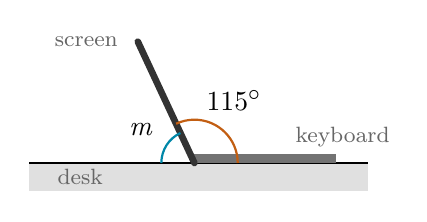
\begin{tikzpicture}[line width=1pt]
    \coordinate (O) at (0,0); \coordinate (L) at (-1.9,0); \coordinate (R) at (2.0,0);
    \coordinate (P) at (115:1.7);
    \fill[black!12] (-2.1,-0.35) rectangle (2.2,0);
    \draw (-2.1,0) -- (2.2,0);
    \fill[black!55] (0,0) rectangle (1.8,0.12);
    \draw[black!80, line width=2.4pt, line cap=round] (O) -- (P);
    \pic[ang, "$115\dg$", angle radius=0.55cm, angle eccentricity=1.7] {angle = R--O--P};
    \pic[let, "$m$", angle eccentricity=1.9] {angle = P--O--L};
    \node[font=\footnotesize, text=black!60, anchor=west] at (1.15,0.33) {keyboard};
    \node[font=\footnotesize, text=black!60, anchor=east] at ($(P)+(-0.12,0)$) {screen};
    \node[font=\footnotesize, text=black!60] at (-1.45,-0.18) {desk};
  \end{tikzpicture}
  \par\vspace{4pt}\raggedright
  \textbf{(a)} Mr Bowen opens his laptop. The screen makes 115\textdegree\ with the
  keyboard. The desk is a straight line. Find $m$.
  \par\vspace{8pt}\textbf{Calculation:} \blank[2.6cm] \ $m =$ \blank[1.4cm]
\end{minipage}\hfill
\begin{minipage}[t]{0.48\textwidth}\centering
  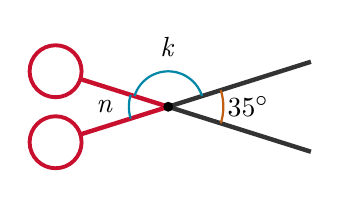
\begin{tikzpicture}[line width=1pt]
    \coordinate (O) at (0,0);
    \coordinate (B1) at (17.5:1.9); \coordinate (B2) at (-17.5:1.9);
    \coordinate (H1) at (197.5:1.15); \coordinate (H2) at (162.5:1.15);
    \draw[black!80, line width=1.6pt] (O) -- (B1); \draw[black!80, line width=1.6pt] (O) -- (B2);
    \draw[cbred, line width=1.6pt] (O) -- (H1); \draw[cbred, line width=1.6pt] (O) -- (H2);
    \draw[cbred, line width=1.4pt] ($(197.5:1.5)$) circle (0.33);
    \draw[cbred, line width=1.4pt] ($(162.5:1.5)$) circle (0.33);
    \pic[ang, "$35\dg$", angle radius=0.7cm, angle eccentricity=1.45] {angle = B2--O--B1};
    \pic[let, "$n$", angle radius=0.5cm, angle eccentricity=1.6] {angle = H2--O--H1};
    \pic[let, "$k$", angle radius=0.45cm, angle eccentricity=1.7] {angle = B1--O--H2};
    \fill (O) circle (1.8pt);
  \end{tikzpicture}
  \par\vspace{4pt}\raggedright
  \textbf{(b)} Mr Bowen's scissors are two straight lines that cross. The blades are
  open at 35\textdegree.
  \par\vspace{6pt}$n =$ \blank[1.4cm] \ because \blank[3.3cm]
  \par\vspace{8pt}$k =$ \blank[1.4cm] \ because \blank[3.3cm]
\end{minipage}
\end{minipage}

% -- X21 --------------------------------------------------------------------
% X12 for angles. Three are wrong, each a different error: a right angle
% treated as 100 (90 + 80 = 170), opposite confused with next-door, and a
% subtraction slip (180 - 75 = 105, not 115). (c) is right.
\qhead[cbgreen]{X21}{Mr Bowen's angle homework}

\noindent\begin{minipage}{\textwidth}
\noindent Circle \textbf{right} or \textbf{wrong}. Write the calculation that shows it.

\vspace{6pt}
{\renewcommand{\arraystretch}{2.0}%
\noindent\begin{tabularx}{\textwidth}{@{}l L C{3.0cm} l@{}}
  \textbf{(a)} & A right angle and 80\textdegree\ make a straight line. & right \sep
    wrong & \blank[3.6cm] \\
  \textbf{(b)} & Two lines cross. One angle is 50\textdegree, so the angle
    \textbf{opposite} it is 130\textdegree. & right \sep wrong & \blank[3.6cm] \\
  \textbf{(c)} & Three angles around a point are 100\textdegree, 120\textdegree\ and
    140\textdegree. & right \sep wrong & \blank[3.6cm] \\
  \textbf{(d)} & On a straight line, one angle is 75\textdegree, so the other is
    115\textdegree. & right \sep wrong & \blank[3.6cm] \\
\end{tabularx}}
\end{minipage}

% -- X22 --------------------------------------------------------------------
% Calculation -> English for an angle: X13 again, for Part 2.
\qhead[cbgreen]{X22}{Now you write the question}

\noindent\begin{minipage}{\textwidth}
\noindent Write a word problem for \quad \expr{180\dg - 65\dg = 115\dg}

\begin{yourturn}[Your word problem must have: tick each one]
  \renewcommand{\arraystretch}{1.35}%
  \begin{tabularx}{\linewidth}{@{}p{0.75cm}L p{0.75cm}L p{0.75cm}L@{}}
    \tickbox & a real thing (a road, a ladder, a door \ldots) & \tickbox & the words
      \textbf{straight line} & \tickbox & full sentences \\
    \tickbox & Mr Bowen & \tickbox & a question at the end & \tickbox & the answer
      115\textdegree \\
  \end{tabularx}
\end{yourturn}
\wlines{4}
\end{minipage}

% ===========================================================================
% ANSWER KEY -- TEACHER COPY ONLY
% ===========================================================================
\ifkey
\clearpage

\hwsection[cbred]{Answer Key --- Teacher Copy}

\linespread{1.0}\selectfont
\setlist[enumerate]{itemsep=2pt, topsep=3pt, leftmargin=*}

\qhead[cbred]{X1}{Make the total}
\noindent (b) 40 \quad (c) 65 \quad (d) 0.6 \quad (e) 0.25 \quad (f) 80 \quad (g) 50
\quad (h) 85 \quad (i) 90

\smallskip
\noindent{\small (e) Expect 0.35 (``75 and 35 make 100'' --- no: 75 + 25) or 0.25
written as 25. (f)--(i) are the angle facts in disguise: the student who finds them
easy already has Part 2.}

\qhead[cbred]{X2}{In your head}
\noindent (b) 2 \quad (c) 5 \quad (d) 5 \quad (e) 1.1 \quad (f) 2.5 \quad (g) 9.9 \quad
(h) 0.75 \quad (i) 5 \quad (j) 4.5 \quad (k) 90 \quad (l) 180

\smallskip
\noindent{\small (e) Expect 0.11 (``9 and 2 make 11''): ten tenths make 1. (g) Expect
9.1 or 10.9. (b), (c), (d), (i) are whole numbers on purpose --- a student who writes
2.0 or 5.0 is right.}

\qhead[cbred]{X3}{Add in columns}
\noindent (b) $358 + 275 = \mathbf{633}$ (carries in the tens and the hundreds) \quad
(c) $409 + 96 = \mathbf{505}$

\smallskip
\noindent{\small (c) is the alignment check. Writing 96 under the 40 of 409 gives 1369;
ones go under ones.}

\qhead[cbred]{X4}{Take away in columns}
\noindent (b) $180 - 74 = \mathbf{106}$ \quad (c) $360 - 145 = \mathbf{215}$

\smallskip
\noindent{\small Both have a 0 in the ones on top. The classic slip is $0 - 4 = 4$
(take the small from the big, whichever row it is in): 180 $-$ 74 then comes out as
114, and 360 $-$ 145 as 225. Ask: ``Can you take 4 from 0?'' --- then exchange a ten.}

\qhead[cbred]{X5}{Add decimals}
\noindent (b) $4.70 + 1.85 = \mathbf{6.55}$ \quad (c) $12.60 + 0.75 = \mathbf{13.35}$

\smallskip
\noindent{\small (c) is empty on purpose: 12.6 needs the tens box, and 0.75's 0 goes in
the ones. A student who writes 12.6 starting in the first box has lined up the left
edge, not the point --- the point is printed, so ask where it is.}

\qhead[cbred]{X6}{Take away decimals}
\noindent (b) $7.40 - 3.18 = \mathbf{4.22}$ \quad (c) $8.00 - 3.25 = \mathbf{4.75}$
\quad (d) $10.0 - 4.6 = \mathbf{5.4}$

\smallskip
\noindent{\small (c) is the one to mark carefully. 5.25 means $8 - 3$ and the .25 copied
down; the orange boxes are there to stop exactly that. (b): 4.38 is ``8 $-$ 0, take the
smaller from the bigger''. (d) needs 10 in the tens and ones boxes.}

\qhead[cbred]{X7}{Bar models}
\noindent (b) $6.0 - 3.8 = \mathbf{2.2}$ \quad (c) $0.75 + 1.25 = \mathbf{2}$ (2.00)
\quad (d) $180 - 65 = \mathbf{115\dg}$

\smallskip
\noindent{\small The picture chooses the operation: whole missing, add; part missing,
take away. Expect $6.0 + 3.8 = 9.8$ in (b) from a student adding every two numbers ---
point at the top bar: 9.8 is bigger than the whole. (d) is Part 2 in a bar.}

\qhead[cbred]{X8}{Number walls}
\noindent (a) middle row 37, 33, 38; \ then 70, 71; \ top \textbf{141}. \\
(b) missing brick $4.25 - 1.5 = \mathbf{2.75}$; \ then $2.75 + 2.25 = 5.00$; \ top
$4.25 + 5.00 = \mathbf{9.25}$.

\smallskip
\noindent{\small (b) is the only take-away: a student who adds $1.5 + 4.25$ for the
missing brick (5.75) gets a wall that does not add up --- ask them to check the brick
above it.}

\qhead[cbred]{X9}{Add or take away?}
\noindent (a) $2.5 + 1.25 = 3.75$ \quad (b) $9.6 - 4.2 = 5.4$ \quad (c) $4.5 + 1.8 =
6.3$ cm \quad (d) $1.5 - 0.35 = 1.15$ litres \quad (e) $2.4 + 3.15 = 5.55$ km \quad
(f) $6 - 2.7 = 3.3$

\smallskip
\noindent{\small \textbf{Mark the calculation first.} (d) Expect 1.25: in $1.50 - 0.35$
the student wrote $0 - 5$ as 5 instead of exchanging. (f) is the trap: $2.7 - 6$ is the English error,
not an arithmetic one --- have them read the Careful line aloud. (c) is HW 12's gecko,
still growing.}

\qhead[cbred]{X10}{Mr Bowen's walk to school}
\noindent (a) $0.75 + 1.3 = \mathbf{2.05}$ km \quad (b) $2.4 - 2.05 = \mathbf{0.35}$ km
\quad (c) $2.05 + 2.05 = \mathbf{4.1}$ km \\
(d) $0.75 + 0.75 + 0.75 + 1.3 = \mathbf{3.55}$ km

\smallskip
\noindent{\small (a) Expect 0.88 from a student who did not line up the points: 1.3 written
under the 75 as if it were 0.13 (1.3 is 1.30). (b) needs (a) first: a student who writes $2.4 - 1.3$ or $2.4 - 0.75$
compared the river with one part of the road. (d) is three walks of 0.75 km, not two:
home to shop, shop to home, home to shop again.}

\qhead[cbred]{X11}{Mr Bowen goes shopping}
\noindent (a) $1.25 + 0.80 = 2.05$ dollars \quad (b) $5.00 - 2.50 = 2.50$ dollars
\quad (c) $1.60 - 0.80 = 0.80$ dollars \\
(d) Step 1: $2.50 + 1.25 + 0.45 = 4.20$; \ Step 2: $5.00 - 4.20 = \mathbf{0.80}$
dollars

\smallskip
\noindent{\small (c) ``How much more'' is a take-away; expect 2.40 from a student who
added. (d) is two steps, the shopping version of X15: a student who stops at 4.20 has
answered ``how much did it cost'', not ``what is his change''.}

\qhead[cbred]{X12}{Mr Bowen's homework}
\noindent (a) wrong, \textbf{6.85} \quad (b) wrong, \textbf{3.6} \quad (c)
\textbf{right} \quad (d) wrong, \textbf{5.75}

\smallskip
\noindent{\small (a) he lined up the right-hand edges, not the points (45 + 235 = 280).
(b) he took 2 from 6 and copied the .4 down. (d) the same error as (b) and X6(c): he
took 3 from 9 and kept the .25. (c) is right so the answer is not ``all wrong''. For the
sentence, accept any one error described in words: \emph{``In (b), Mr Bowen took 2 from
6 and did not take away the 0.4.''}}

\qhead[cbred]{X13}{Now you write the question}
\noindent{\small Check, in order: something Mr Bowen buys for 3.45 dollars; he pays 5
dollars; it asks for the change; a question mark; full sentences. \\
Model: \emph{``Mr Bowen buys a sandwich for 3.45 dollars. He pays with 5 dollars. How
much change does he get?''} \\
The usual failure: a question whose answer is 3.45 (``how much is the sandwich?'') or
8.45 (it adds). Ask the student to answer their own question.}

\qhead[cbred]{X14}{What is left of 180\textdegree?}
\noindent (b) $180 - 110 = \mathbf{70\dg}$ \quad (c) $180 - 72 = \mathbf{108\dg}$ \quad
(d) $180 - 145 = \mathbf{35\dg}$ \quad (e) $180 - 125 = \mathbf{55\dg}$ \quad (f) $180 -
147.5 = \mathbf{32.5\dg}$

\smallskip
\noindent{\small (c) and (e) have the letter on the right. Expect 252 for (c) from a
student who adds. (f) is X6's skill: $180.0 - 147.5$, a 0 after the point.}

\qhead[cbred]{X15}{Two angles, then what is left}
\noindent (b) $35 + 90 = 125$, \ $180 - 125 = \mathbf{55\dg}$ \quad (c) $48 + 75 = 123$,
\ $180 - 123 = \mathbf{57\dg}$

\smallskip
\noindent{\small (b) has no number for the right angle: expect $180 - 35 = 145$ from
anyone who skipped the square.}

\qhead[cbred]{X16}{Straight line or not?}
\noindent $72 + 106 = 178$, \textbf{no} \quad $129 + 51 = 180$, \textbf{yes} \quad
$88.5 + 91.5 = 180$, \textbf{yes} \quad $64 + 117 = 181$, \textbf{no}

\smallskip
\noindent{\small 178 and 181 are the point: ``nearly 180'' is not a straight line. A
``yes'' for either means the student looked instead of adding.}

\qhead[cbred]{X17}{Angles in words}
\noindent (a) $180 - 70 = \mathbf{110\dg}$ \quad (b) $180 \div 2 = \mathbf{90\dg}$
\quad (c) $50 + 60 = 110$, \ $180 - 110 = \mathbf{70\dg}$ \quad (d) $180 - 90 =
\mathbf{90\dg}$ \quad (e) $360 - 200 = \mathbf{160\dg}$

\smallskip
\noindent{\small Every one is decided by its English. (b) ``equal'' is the only divide;
expect 180 from a student who missed it. (d) ``right angle'' is the 90 they must supply.
(e) ``full turn'' is 360: expect $180 - 200$ (impossible) from a student who uses 180
for everything.}

\qhead[cbred]{X18}{Two lines cross}
\noindent (a) $t = 40\dg$ (opposite), \ $s = u = 140\dg$ ($180 - 40$) \quad (b) $w =
115\dg$ (opposite), \ $v = x = 65\dg$ ($180 - 115$)

\smallskip
\noindent{\small (b) gives only one angle. A student who writes 115 for all three has
called every angle ``opposite''; $v$ is \emph{next to} 115\textdegree.}

\qhead[cbred]{X19}{Around a point}
\noindent (a) $150 + 125 = 275$, \ $360 - 275 = \mathbf{85\dg}$ \quad (b) $90 + 140 =
230$, \ $360 - 230 = \mathbf{130\dg}$

\smallskip
\noindent{\small Expect $180 - 275$ (impossible) from a student who uses 180 everywhere:
ask ``line or point?''. (b) has a square for the 90.}

\qhead[cbred]{X20}{Mr Bowen's angles}
\noindent (a) $180 - 115 = \mathbf{65\dg}$ \quad (b) $n = \mathbf{35\dg}$ because
opposite angles are equal; \ $k = \mathbf{145\dg}$ because next-door angles make
$180\dg$ ($180 - 35$).

\smallskip
\noindent{\small (a) is X14 with a picture. (b): $n$ is between the handles, $k$ between
a blade and a handle. Accept the reason in the student's own words.}

\qhead[cbred]{X21}{Mr Bowen's angle homework}
\noindent (a) \textbf{wrong}: $90 + 80 = 170$, not 180 \quad (b) \textbf{wrong}:
opposite angles are equal, so it is $50\dg$ ($130\dg$ is next to it) \\
(c) \textbf{right}: $100 + 120 + 140 = 360$ \quad (d) \textbf{wrong}: $180 - 75 = 105$,
not 115

\smallskip
\noindent{\small Three different errors on purpose: (a) forgets that a right angle is a
number (90), (b) swaps opposite and next-door, (d) is an arithmetic slip that ``looks
about right''. A student who marks (c) wrong probably added to 180: ``around a point''
is 360.}

\qhead[cbred]{X22}{Now you write the question}
\noindent{\small Check, in order: a straight line (named); one angle of 65\textdegree;
it asks for the other angle; a question mark; full sentences. \\
Model: \emph{``Mr Bowen leans a ladder on a wall. The ladder makes 65\textdegree\ with
the ground. The ground is a straight line. What is the angle on the other side of the
ladder?''} \\
The usual failure: a question whose answer is 65\textdegree\ (it gives 115 and asks
for 65 --- still a good question, but not this one) or one about a point (360).}

\fi

\end{document}
